\chapter{Chiffrement et Protocoles}

\section{Définitions et contexte}

Nous allons tout d'abord apporter quelques précisions au contexte dans lequel nous travaillons. Plusieurs failles ont été trouvées sur RSA-OAEP ainsi que sur le mode CBC. Nous allons donc décrire ces deux principes.
\subsection{OAEP : \textit{Optimal Asymmetric Encryption Padding}}
Dans les chiffrements par blocs, cela nécessite généralement que tous les blocs soient d'une taille précise. Or ce n'est pas toujours le cas. Pour cela, on rajoute des bits de bourrage (padding).\\
OAEP est un schéma de remplissage, généralement utilisé avec RSA (en prétraitement). Il a été introduit en 1994 par Mihir Bellare et Phil Rogaway1. L'OAEP est une forme de réseau de Feistel qui nécessite une source d'aléa ainsi que deux fonctions de hachage.\\
RSA-OEAP peut être prouvé sûr dans un modèle théorique idéalisé, celui de l'oracle aléatoire. Il est recommandé par les PKCS.\\
OAEP a deux buts :
\begin{itemize}
\item insérer un élément d'aléatoire qui permet de passer d'un schéma déterministe à un schéma non déterministe (le même message clair chiffré deux fois avec la même clef et le même algorithme n'aura pas le même message chiffré.)
\item prévenir un déchiffrement partiel en s'assurant que l'attaquant ne peut retrouver une portion du text clair sans être capable d'inverser la fonction trapdoor (par exemple la factorisation de deux grands nombres premiers : il est facile de multiplier, mais quand on n'a que le produit il est très difficile de retrouver les facteurs).\\
\end{itemize}
Il n'est pas pouvé sûr pour une attaque IND-CCA (attaque à texte chiffré seulement). Victor Shoup a démontré qu'il n'existe pas de preuve générale.
Il a montré que dans un cas IND-CCA, quelqu'un qui sait comme inverser partiellement une primitive d'insertion mais ne sait pas comment l'inverser complètement, pourrait bien être en mesure de casser le système. Par exemple, on peut imaginer quelqu'un qui peut attaquer RSAES-OAEP si on sait comment retrouver tous les octets exceptés les 20 premiers d'un entier généré aléatoirement chiffré avec RSAEP. Un tel attaquant n'a pas besoin d'être cacpable d'inverser entièrement RSAEP (RSA Encryption Protocole), parce qu'il n'utilise pas les 20 premiers octets dans son attaque.

\subsubsection*{Réseau de Feistel}
Il est utilisé dans les systèmes de chiffrement par bloc. Un réseau de Feistel repose sur des principes simples dont des permutations, des substitutions, des échanges de blocs de données et une fonction prenant en entrée une clé intermédiaire à chaque étage.\\
\begin{figure}[H]
\centering
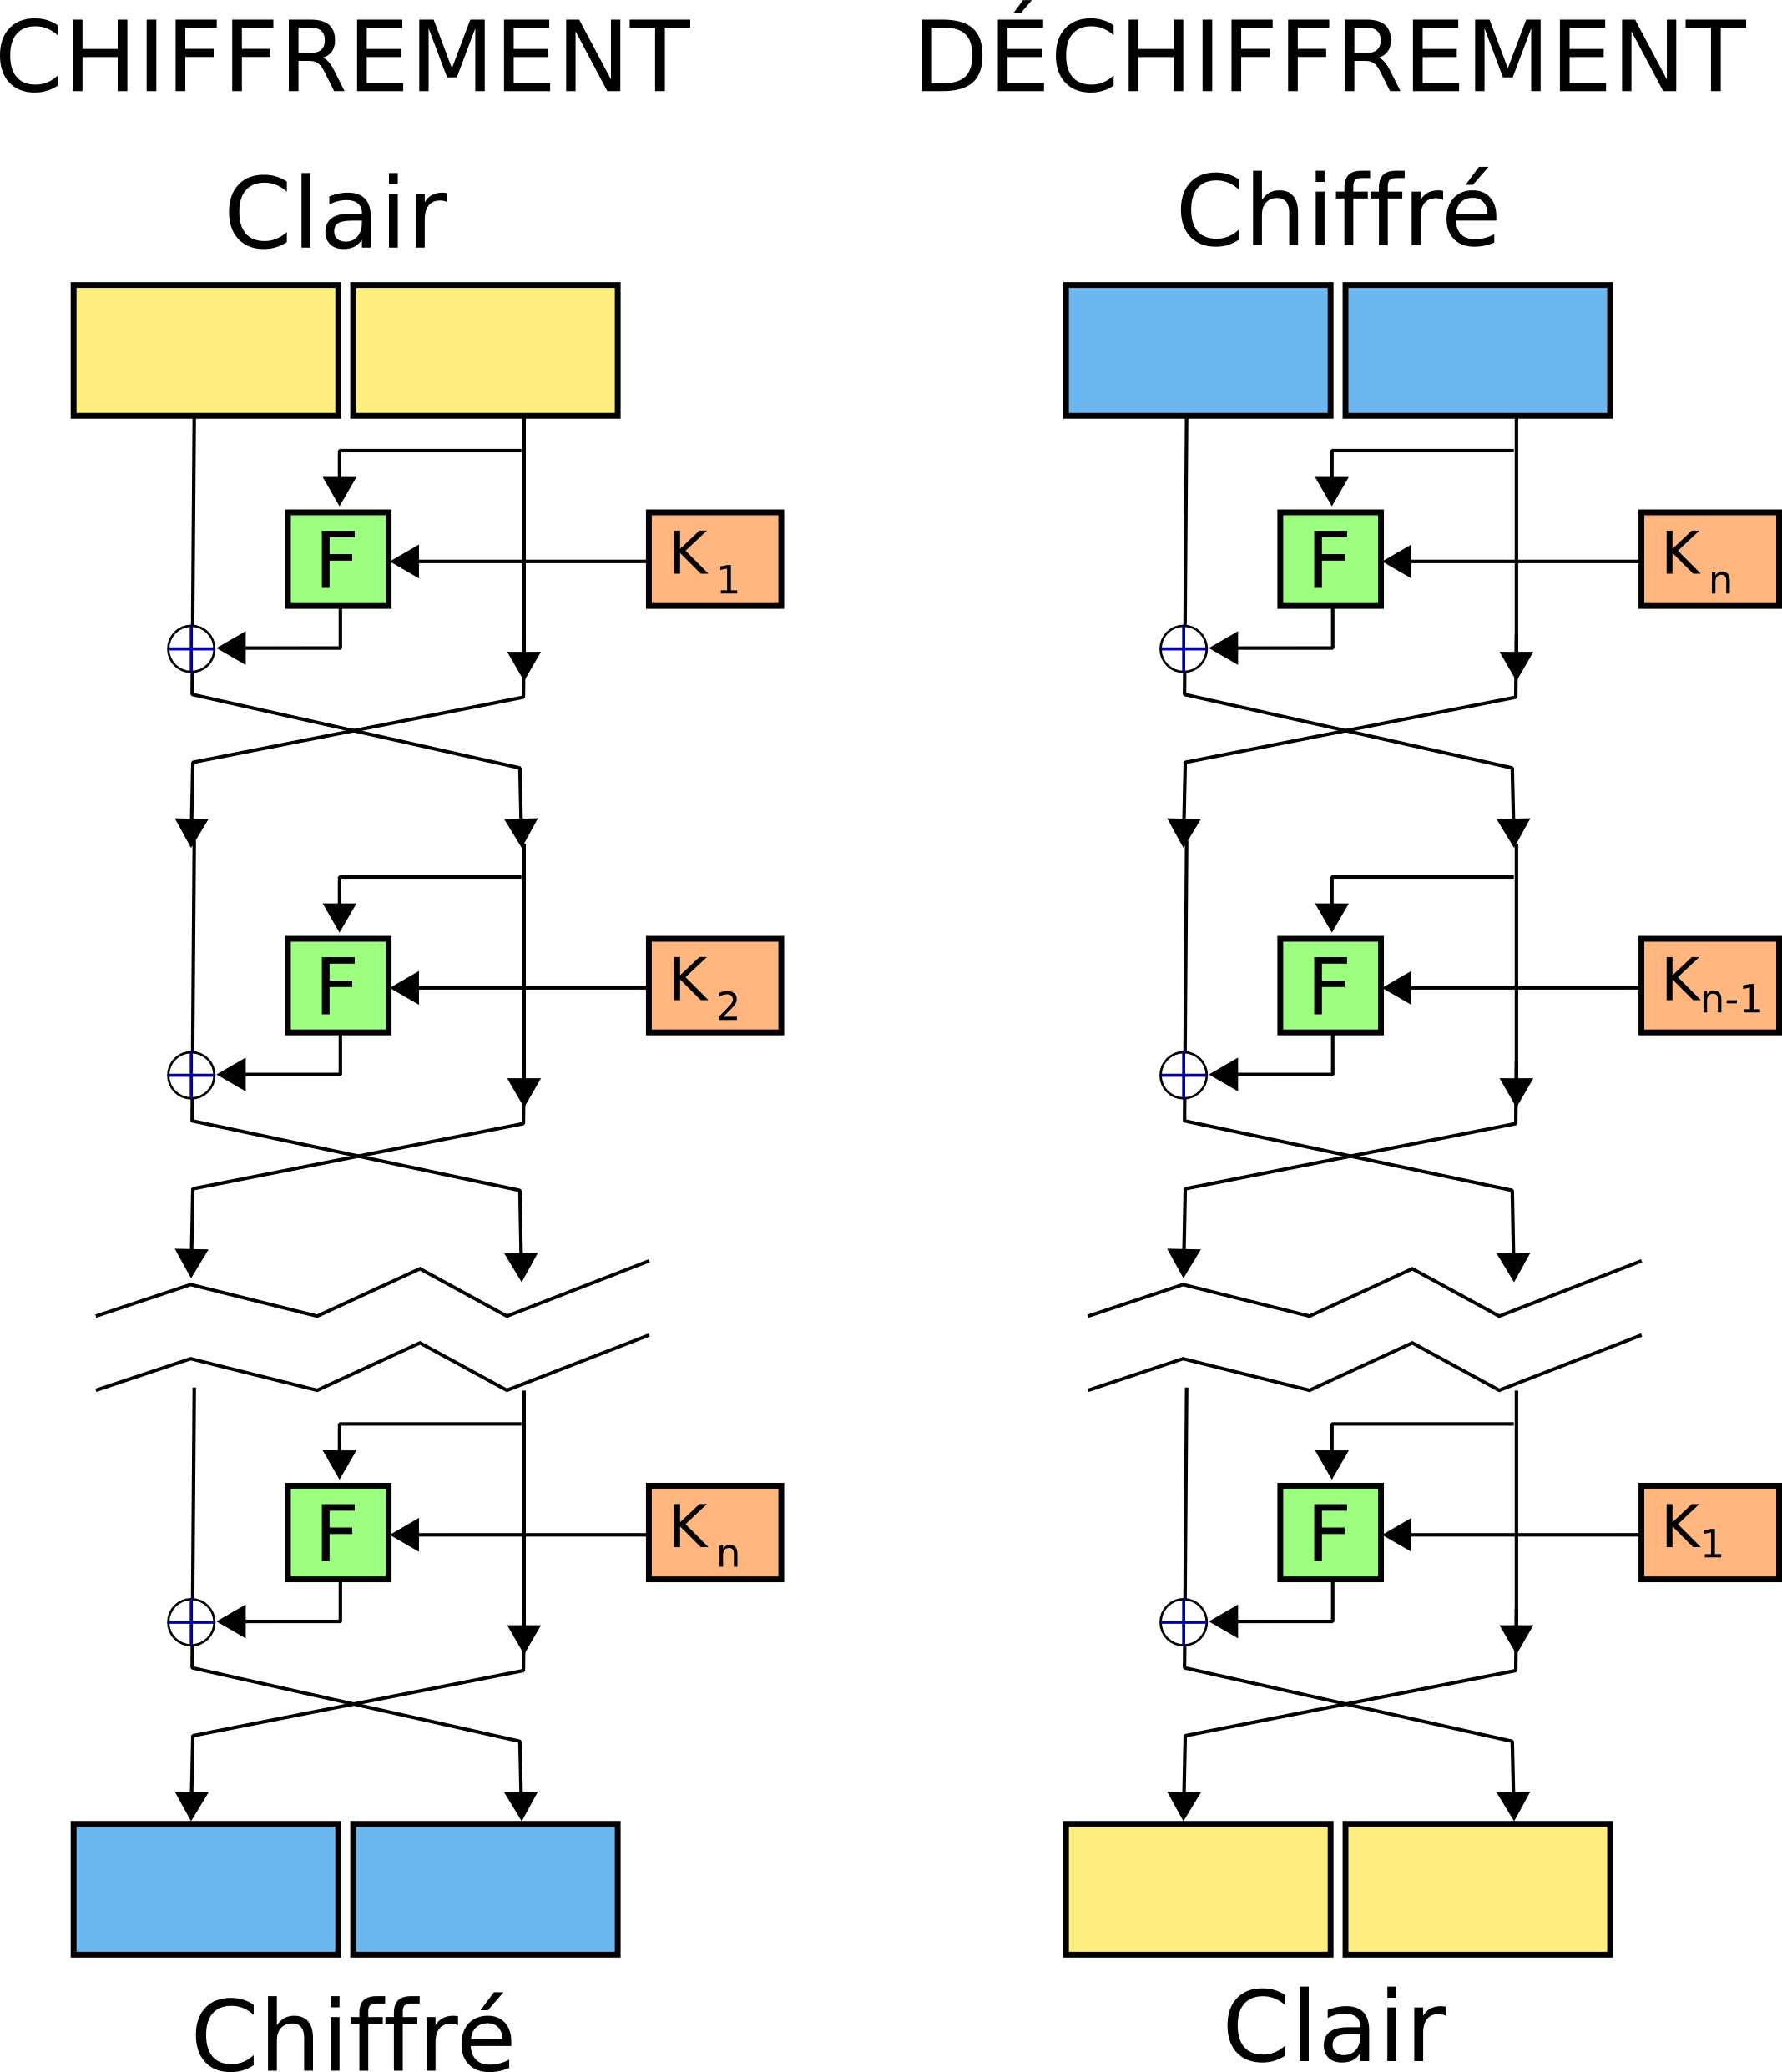
\includegraphics[width=7cm]{images/Reseau_de_feistel.png}
\caption{Réseau de Feistel}
\label{Feistel}
\end{figure}

Le chiffrement DES par exemple repose sur ce réseau, et effectue 16 tours.\\
Généralement les deux parties sont équilibrées même si par exemple des algorithme comme MacGuffin de Bruce Schneier utilise un réseau non équilibré.

\subsection{RSA-OAEP}
Dans la PKCS\#1 est décrit le standard de RSA-OAEP. RSAES-OAEP est le terme plus facilement utilisé dans le document : RSA Encryption Scheme OAEP.\\
Il regroupe les primitives RSAEP et RSADP : respectivement RSA Encryption Protocole et RSA Decryption Protocole.

\subsubsection{RSAES-OAEP-ENCRYPT}
Options :
\begin{description}
\item [Hash :] fonction de hachage (\texttt{hLen} contient la longueur en octets de la sortie de fonction de hachages);
\item [MGF :] fonction de génération de masque.\\
\end{description}
Entrée :
\begin{description}
\item [(n, e) : ] destinataire de la clef publique RSA (\texttt{k} contient la longueur en octets du modulo RSA \texttt{n});
\item [M : ] message à chiffrer, un chaîne d'octets de longueur \texttt{mLen}, quand \texttt{mLen <= k - 2hLen - 2};
\item [L : ] champ optionnel à associer au message, la valeur par défaut pour \texttt{L}, si \texttt{L} n'a aucune condition, est la chaîne vide.\\
\end{description}
Sortie :
\begin{description}
\item [C : ] texte chiffré, une chaîne d'octets de longueur \texttt{k}.\\
\end{description}
Erreurs :
\begin{itemize}
\item "\textit{message too long}";
\item "\textit{label too long}".\\
\end{itemize}
Précondition :
\begin{itemize}
\item la clef publique RSA \texttt{(n, e)} est valide.\\
\end{itemize}
Étapes:
\begin{enumerate}
\item vérifier de la longueur:
\begin{enumerate}
\item si la longueur de \texttt{L} est plus grande que la longueur limite en entrée de la fonction de hachage ($2^{61} - 1$ octets pour SHA-1), renvoyer "\textit{label too long}" et arrêter;
\item si \texttt{mLen > k - 2hLen - 2}, le message "\textit{message too long}" est renvoyé et la fonction est stoppée.\\
\end{enumerate}
\item coder EME-OAEP (voir Figure 1 ci-dessous):
\begin{enumerate}
\item si l'étiquette \texttt{L} n'est pas spécifiée, laisser \texttt{L} à une chaîne vide. Laisser \texttt{lHash = Hash(L)}, une chaîne d'octets de taille \texttt{hLen} (voir note plus bas);
\item générer une chaîne d'octets PS consistant en \texttt{k - mLen - 2hLen - 2} d'octets zéro. La taille de \texttt{PS} peut être zéro;
\item concaténer \texttt{lHash}, \texttt{PS}, un unique octet avec la valeur hexadécimale \textit{0x01}, et le message \texttt{M} pour former un bloc de données DB de longueur \texttt{k - hLen - 1} octets, tel que : \texttt{DB} = \texttt{lHash} \textbar\textbar \texttt{PS} \textbar\textbar \textit{0x01} \textbar\textbar \texttt{M};
\item générer un une chaîne d'octets aléatoires de longueur \texttt{hLen};
\item laisser \texttt{dbMask = MGF(seed, k - hLen - 1)};
\item laisser \texttt{maskedDB = DB xor dbMask};
\item laisser \texttt{seedMask = MGF(maskedDB, hLen)};
\item laisser \texttt{maskedSeed = seed xor seedMask};
\item concaténer un unique octet avec la valeur hexadécimale \textit{0x00}, \texttt{maskedSeed}, et \texttt{maskedDB} pour former un message chiffré \texttt{EM} de longueur \texttt{k} octets tel que \texttt{EM = 0x00} \textbar\textbar \texttt{maskedSeed} \textbar\textbar \texttt{maskedDB}.\\
\end{enumerate}
\item chiffrement RSA :
\begin{enumerate}
\item convertir le message codé \texttt{EM} en un entier représentatif du message \texttt{m} (voir section 4.2) : \texttt{m = OS2IP (EM)};
\item appliquer la primitive de chiffrement \texttt{RSAEP}(Section 5.1.1) avec la clef RSA publique (n, e) pour produire un entier c représentatif du message chiffré : \texttt{c = RSAEP ((n, e), m)};
\item convertir le texte chiffré représentatif \texttt{c} en un texte chiffré \texttt{C} de taille \texttt{k} octets (voir Section 4.1) : \texttt{C = I2OSP (c, k)}.\\
\end{enumerate}
\item envoyer en sortie le texte chiffré \texttt{C}.\\
\end{enumerate}
\paragraph{Note} Si \texttt{L} est une chaîne vide, la valeur du hash correspondante \texttt{lHash} a la représentation hexadécimale suivante pour différents choix de hash :


\begin{table}[H]
\centering
\begin{tabularx}{17cm}{Xllllll}
SHA-1: & (0x)da39a3ee & 5e6b4b0d & 3255bfef & 95601890 & afd80709 & \\
SHA-256: & (0x)e3b0c442 & 98fc1c14 & 9afbf4c8 & 996fb924 & 27ae41e4 & 649b934c\\
& a495991b & 7852b855 & & & &\\
SHA-384: & (0x)38b060a7 & 51ac9638 & 4cd9327e & b1b1e36a & 21fdb711 & 14be0743\\
& 4c0cc7bf & 63f6e1da & 274edebf & e76f65fb & d51ad2f1 & 4898b95b\\
SHA-512: & (0x)cf83e135 & 7eefb8bd & f1542850 & d66d8007 & d620e405 & 0b5715dc\\
& 83f4a921 & d36ce9ce & 47d0d13c & 5d85f2b0 & ff8318d2 & 877eec2f\\
& 63b931bd & 47417a81 & a538327a & f927da3e &	&\\
\end{tabularx}
\caption{Représentations hexadécimales}
\label{repres_hexa}
\end{table}

\begin{description}
    \item SHA-1: (0x)da39a3ee 5e6b4b0d 3255bfef 95601890 afd80709;
    \item SHA-256: (0x)e3b0c442 98fc1c14 9afbf4c8 996fb924 27ae41e4 649b934c\\
                a495991b 7852b855;
    SHA-384: (0x)38b060a7 51ac9638 4cd9327e b1b1e36a 21fdb711 14be0743\\
                4c0cc7bf 63f6e1da 274edebf e76f65fb d51ad2f1 4898b95b;
    SHA-512: (0x)cf83e135 7eefb8bd f1542850 d66d8007 d620e405 0b5715dc\\
                83f4a921 d36ce9ce 47d0d13c 5d85f2b0 ff8318d2 877eec2f\\
                63b931bd 47417a81 a538327a f927da3e.\\
\end{description}

\begin{figure}[H]
\centering
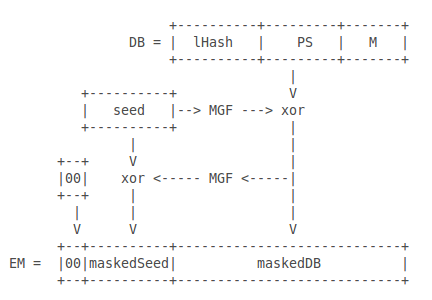
\includegraphics[width=10cm]{images/schema.png}
\caption{Opération de chiffrement EME-OAEP}
\label{fig21}
\end{figure}

\texttt{lHash} est le hash de l'étiquette optionnelle \texttt{L}. L'opération de déchiffrement suivant inverse les étapes pour retrouver \texttt{M} et vérifier \texttt{lHash} et \texttt{PS}.


\subsubsection{RSAES-OAEP-DECRYPT (K, C, L)}

Options :
\begin{description}
\item [Hash :] fonction de hachage (\texttt{hLen} contient la longueur en octets de la sortie de la fonction de hachage);
    \item [MGF :] fonction de génération du masque.\\
\end{description}
Entrée :
\begin{description}
    \item [K :] destinataire de la clef privée RSA (\texttt{k} contient la longueur en octets du modulo RSA \texttt{n});
    \item [C :] texte chiffré à déchiffrer, une chaîne de caractères de taille \texttt{k}, où \texttt{k = 2hLen + 2};
    \item [L :] champ optionnel dont l'association avec le message doit être garantie; la valeur par défaut pour \texttt{L} est, si pas de spécification, une chaîne vide.\\
\end{description}
Sortie :
\begin{description}
    \item [M :] message, une chaîne d'octets de longueur \texttt{mLen}, où \texttt{mLen <= k - 2hLen - 2}.\\
\end{description}
Erreur :
\begin{itemize}
\item "decryption error";
\end{itemize}
Étapes :
\begin{enumerate}
\item Vérification des longueurs :
\begin{enumerate}
      \item Si la longueur de \texttt{L} est supérieur à la taille limite en entrée de la fonction de hachage (\texttt{$2^{61 - 1}$} octets pour SHA-1), renvoie "decryption error" et s'arrête;
\item Si la longueur du texte chiffré \texttt{C} n'est pas de \texttt{k} octets, renvoie "decryption error" et s'arrête;
     \item Si \texttt{k < 2hLen + 2}, renvoie "decryption error" et s'arrête.\\
\end{enumerate}
\item déchiffrement RSA :
\begin{enumerate}
      \item Convertir le texte chiffré \texttt{C} en un entier \texttt{c} représentatif du message chiffré (voir Section 4.2) : \texttt{c = OS2IP (C)};
      \item Appliquer la primitive de déchiffrement \texttt{RSADP} à la clef privée RSA \texttt{K} et au message chiffré représentatif \texttt{c} pour produire un entier \texttt{m} représentatif du message clair : \texttt{m = RSADP (K, c)};\\
       si RSADP renvoie "ciphertext representative out of range" (signifie que \texttt{c >= n}), renvoie "decryption error" et s'arrête;
       \item convertir le message représentatif \texttt{m} en un un message déchiffré \texttt{EM} de longueur \texttt{k} octets (voir Section 4.1) : \texttt{EM = I2OSP (m, k)}.\\
\end{enumerate}
\item déchiffrement EME-OAEP :
\begin{enumerate}
      \item si l'étiquette \texttt{L} n'est pas spécifiée, laisser \texttt{L} à une chaîne vide, laisser \texttt{lHash = Hash(L)}, une chaîne d'octets de longueur \texttt{hLen}
       \item séparer le message encodé \texttt{EM} dans un seul octet \texttt{Y}, une chaîne d'octets \texttt{maskedSeed} de longueur \texttt{hLen}, et une chaîne d'octets \texttt{maskedDB} de longueur \texttt{k - hLen - 1} telle que \texttt{EM = Y \textbar\textbar maskedSeed \textbar\textbar maskedDB};
       \item laisser \texttt{seedMask = MGF(maskedDB, hLen)};
       \item laisser \texttt{seed = maskedSeed xor seedMask};
       \item laisser \texttt{dbMask = MGF(seed, k - hLen - 1)};
       \item laisser \texttt{DB = maskedDB xor dbMask};
       \item séparer \texttt{DB} en une chaîne d'octet \texttt{lHash} de longueur \texttt{hLen}, une chaîne de padding (possiblement vide) \texttt{PS} consistant en des octets hexadécimaux de valeur \textit{0x00}, et un message \texttt{M} tel que \texttt{DB = lHash \textbar\textbar PS \textbar\textbar 0x01 \textbar\textbar M};
\\ s'il n'y a pas d'octet avec la valeur hexadécimale \textit{0x01} pour séparer \texttt{PS} de \texttt{M}, si \texttt{lHash} n'est pas égal à \texttt{lHash}, ou si \texttt{Y} n'est pas une sortie non nulle, renvoyer "decryption error" et s'arrêter.\\
\end{enumerate}
\item Renvoyer le message M.\\
\end{enumerate}
\paragraph{Note} Il faut faire attention qu'un adversaire ne puisse distinguer les différentes erreurs dans les conditions de l'étape 3, que ce soit par un message d'erreur, ou un temps de réponse différent, ou, plus généralement, apprendre une information partielle à propos du message en clair \texttt{EM}. Sinon un adversaire peut être en mesure d'obtenir des informations utiles sur le déchiffrement du texte chiffré \texttt{C}, conduisant à une attaque à chiffré choisi telle que celle observée par Manger.
   
\subsubsection{RSAES-PKCS1-v1\_ 5}

   RSAES-PKCS1-v1\_5 combine les primitives RSAEP et RSADP avec la méthode de codage EME-PKCS1-v1\_ 5. Il est mathématiquement équivalent au schéma de chiffrement dans la PKCS \# 1 v1.5. RSAES-PKCS1-v1\_ 5 peut fonctionner sur des messages de longueur supérieure à \texttt{k - 11} octets (\texttt{k} est la longueur en octets du modulo RSA), bien qu'il faille faire attention aux attaques portant sur les faibles exposants RSA menée par Coppersmith, Franklin, Patarin, and Reiter quand les longs messages sont chiffrés (voir le troisième point dans les notes ci-dessous).\\
En règle générale, l'utilisation de ce schéma pour chiffrer un message arbitraire, en opposition à une clef générée aléatoirement, n'est pas recommandé.\\
Il est possible de générer des textes chiffrés RSAES-PKCS1-v1\_5 valides sans connaître les messages clairs correspondants, avec une probabilité raisonnable de réussite.\\
Cette possibilité peut être exploitée dans une attaque à chiffré choisi, comme montré en [6]. Par conséquent, si RSAES-PKCS1-v1\_5 doit être utilisé, certaines contre mesures faciles à implémenter devraient être mises en place afin de contrecarrer l'attaque trouvée en [6].\\
Des exemples typiques comprennent l'ajout de la structure des données à encoder, le contrôle rigoureux de la conformité des PKCS\# 1v1.5 (et d'autres redondance) dans les messages déchiffrés, et la consolidation des messages d'erreur dans un protocole client-serveur basée sur PKCS \# 1 v1.5. Ils peuvent tous être des contre-mesures efficaces et n'entraînent pas de changement à un protocole n\degres 1 sur la base de v1.5-PKCS. Il a été récemment montré que la sécurité du protocole SSL / TLS handshake, qui utilise RSAES-PKCS1-v1\_5 et certaines contre-mesures, peut être liée à une variante du problème RSA.\\
  
\paragraph{Note} Les passages suivants décrivent des recommandations concernant l'utilisation de RSAES-PKCS1-v1\_5. Les recommandations de la version 1.5 de ce document sont inclues ainsi que de nouvelles recommandations motivées par les avancées de cryptanalyse durant les années suivantes.
\begin{itemize}
\item il est recommandé que les octets pseudo aléatoires soient générés indépendamment pour chaque processus de chiffrement, en particulier si la même donnée est en entrée pour plus d'un processus de chiffrement. Les résultats de Haastad sont une des motivations pour cette recommandation;
\item La chaîne de padding \texttt{PS} est d'une longueur d'au moins 8 octets, ce qui est une condition de sécurité pour les opérations sur les clefs publiques, et qui rend difficile pour les attaquants de récupérer les données en essayant tous les blocs chiffrés possibles.
\item les octets pseudo aléatoires peuvent aussi aider à contrecarrer une attaque grâce à Coppersmith et al. quand la taille du message à chiffrer est gardé petit. L'attaque marche sur les petits exposants RSA quand des messages similaires sont chiffrés avec la même clef publique. Plus spécifiquement, une façon peut être, quand deux entrées RSAEP correspondent sur une large portion de bits (8/9) et qu'un petit exposant RSA est utilisé (e = 3) pour chiffrer les deux, il peut être possible de retrouver les entrées avec l'attaque. Une autre façon d'attaquer est couronnée de succès pour déchiffrer un seul texte chiffré, quand une large proportion (2/3) des entrées de RSAEP est déjà connue. Pour des applications typiques, le message à chiffrer est court (par exemple une clef symétrique de 128 bits) donc peu d'informations seront connues ou en commun entre deux messages pour permettre l'attaque. Cependant, si un long message est chiffré, ou si une partie du message est connu, alors l'attaque peut fonctionner. Dans tous les cas, le schéma RSAES-OAEP surmonte l'attaque.\\
\end{itemize}

\subsection{CBC : \textit{Cipher Block Chaining}}
C'est un mode de chiffrement qui a été très utilisé : enchaînement des blocs.\\
Sur chaque bloc, un OU exclusif avec le chiffrement du bloc précédent est appliqué. Un vecteur d'initialisation est lui aussi utilisé. Contrairement au mode ECB, les blocs identiques ne seront pas chiffrés de la même façon. On ne pourra donc pas repérer de chaîne de caractères récurrentes aussi facilement. Ce mode de chiffrement possède plusieurs inconvénients :
\begin{itemize}
\item un chiffrement de plusieurs blocs en parallèles est impossible (puisque chaque bloc dépend du chiffrement du précedent). Déchiffrer avec un IV incorrect entraînera une corruption dans le premier bloc en clair, mais les blocks suivants seront corects. C'est parce qu'un texte claire peut être récupéré grâce à deux blocs adjacents du texte chiffré. Le déchiffrement, contrairement au chiffrement, peut donc être parallélisé. À noter que si un seul bit change dans le texte chiffré, le bloc clair correspondant est complètement corrompu.
\item Si une erreur se produit sur un bloc, elle sera répercutée sur tous les suivants. La propagation d'erreur n'est pas limitée.
\end{itemize}
\begin{figure}[H]
\centering
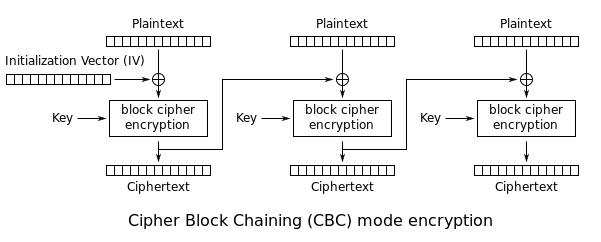
\includegraphics[width=13cm]{images/CBC_chiff.png}
\caption{Chiffrement CBC}
\label{CBC_chiff}
\end{figure}

\begin{figure}[H]
\centering
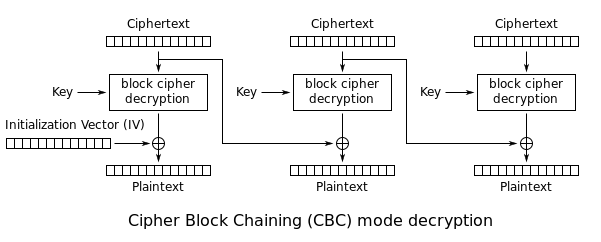
\includegraphics[width=13cm]{images/CBC_dechiff.png}
\caption{Déchiffrement CBC}
\label{CBC_dechiff}
\end{figure}

Il a d'abord été défini par le NIST dans le FIPS 81 (\url{http://www.itl.nist.gov/fipspubs/fip81.htm}). Le standard a été publié en 1981.


\section{Audits}
\subsection{Audit 3.1 : Les "Manger's attack" sur RSA-OAEP}
\subsubsection{Normes visées}

A remplir.

\subsubsection{Faille}

RSA-OAEP peut être soumis à une attaque nommée "Mangers Attack" selon son implantation \cite{mangers2010falko}. OpenSSL semble être vulnérable à une attaque de ce type, à base de "prédictions" par injections de fautes. La vulnérabilité semble être très récente puisqu'elle fonctionne sous OpenSSL 1.0.0.\\


Le padding OAEP devait pallier le problème d'insécurité que causait le padding PKCS\#1 v1.5 (attaque à chiffré choisi) \cite{bleichenbacherPCKS}. OpenSSL a tout de même pris en compte cette vulnérabilité et a placé des contres-mesures efficaces. La Technische Universität Darmstadt (Allemagne) explique en détail comment sont implémentées ces contres-mesures et montre que dans certains cas l'attaque reste possible. Enfin, elle apporte ses propres contre-mesures.\\

On peut noter que plusieurs librairies sont vulnérables à une attaque de Manger qui consiste à contrôler la taille des paramètres à haché, mais que l'implantation de RSA-OAEP d'OpenSSL ne le permet pas.La raison est que le décodage OAEP est linéaire quelque soit la taille des paramètres et les erreurs survenues. Il semble également y avoir un problème avec l'OAEP\_padding sur le chiffrement RSA. Bill Nickless recommande l'utilisation de PKCS\_padding. \cite{sourceforgeRSAbroken}	\\


\subsubsection{Implémentation}

\paragraph{Configuration visée.\\}

L'étude a été réalisée sur la librairie OpenSSL-1.0.0.

\paragraph{Fonction.\\}

La fonction auditée se nomme RSA\_padding\_check\_PKCS1\_OAEP() (cf. \textit{Listing} \ref{rsaoaep}) et est accessible à partir du chemin \texttt{openssl/crypto/rsa/rsa\_oaep.c}.


\begin{lstlisting}[style=customc,caption=rsa\_oaep.c,
label=rsaoaep]
lzero = num - flen;
if (lzero < 0)
{
/* signalling this error immediately after detection might allow
* for side-channel attacks (e.g. timing if 'plen' is huge
* -- cf. James H. Manger, "A Chosen Ciphertext Attack on RSA
Optimal
* Asymmetric Encryption Padding (OAEP) [...]", CRYPTO 2001),
* so we use a 'bad' flag */
bad = 1;
lzero = 0;
flen = num; /* don't overflow the memcpy to padded_from */
}
\end{lstlisting}

Le développeur n'a pas considéré qu'il y avait un grand danger dans le code de contre-mesures.\\
Pourtant l'étude confirme qu'il y a un décalage de temps possible, certes léger mais qui peut entraîner une attaque en "branch prediction" (qui peut se traduire en prédiction par dérivation).\\

\subsubsection{Conclusion}

Il n'y a pas vraiment de quoi s'alarmer, cette attaque est en pratique infaisable sur un serveur car il y a suffisamment de variations de délais (différences de CPU, opérations multi-tâches, connexions réseaux, etc...) pour éviter une attaque par timing. Cependant, sur des systèmes embarqués l'attaque peut être réalisable, et il serait plus prudent de pallier ce problème.

\subsection{Audit 3.2 : Chiffrement SSLv3 ou TLS 1.0 en mode CBC}
\subsubsection{Normes visées}

A remplir.

\subsubsection{Description de la faille}

En Septembre 2011, une attaque en man in the middle très efficace a vu le jour contre les protocoles SSLv3 et TLS 1.0. \cite{ekr2011beast} \cite{imperial2011beast} \cite{goodin2011beast} \cite{gallagher2011beast}. L'attaque est à clair choisi. Le but étant d'insérer des morceaux de texte clair grâce au navigateur dans la requête chiffrée avec ces protocoles, ceci afin de récupérer les cookies de session.\\

La technique est basique, un individu enregistre plusieurs cookies de session auprès de divers sites officiels (banques, messageries, etc...). Puis, il clique malencontreusement sur du code Java malveillant (publicité, image, etc...). et l'attaque se déroule automatiquement. L'ensemble des cookies est envoyé au serveur malveillant qui n'a plus qu'à déchiffrer les clés de session.\\

La cause viendrait du mode de chiffrement choisi : CBC. SSL/TLS est un protocole qui chiffre un canal de communication. De ce fait il ne chiffre pas un fichier unique, mais une série d'enregistrements. Il y a deux façons d'utiliser le mode CBC dans ce cas précis :
\begin{itemize}
\item Prendre chacun de ces enregistrements indépendamment des autres. Générer un nouveau vecteur d'initialisation à chaque fois.
\item Traiter ces enregistrements comme un seul objet en les concaténant. Le vecteur d'initialisation est donc choisi aléatoirement pour le premier enregistrement et pour les autres, il aura pour valeur le dernier bloc de l'enregistrement précédent.\\

\end{itemize}

SSLv3 et TLS 1.0 utilisent ce deuxième choix, cela soulève un lourd problème de sécurité. En 2004, Moeller \cite{moeller2004cbc} trouve une méthode pour exploiter ce mauvais choix afin de récupérer des morceaux de textes clairs. Il y a certes une faille immense, mais peu exploitable. Les grandes entreprises savent (normalement) qu'il ne faut pas utiliser le mode CBC pour du chiffrement SSL/TLS. Et, dans tout les cas, plusieurs navigateurs ne permettent pas ce type d'attaque (c'est le cas de Chrome par exemple).

\subsubsection{Tests}

Nous n'avons pas repris les tests du logiciel BEAST qui s'avère être introuvable sur le Web (celui-ci étant un projet universitaire, développé par un étudiant de l'Université de Versailles). Mais une vidéo de l'exploit est accessible sur YouTube au lien ci-dessous : \\

\textbf{Lien YouTube : } \href{http://www.youtube.com/watch?v=ujz4SXzWK9o} {http://www.youtube.com/watch?v=ujz4SXzWK9o}

\subsubsection{Recommandations}

La faille existe tant que l'association de ces protocoles avec le mode de chiffrement CBC existe. Même si l'attaque est infaisable sur les navigateurs les plus répandus (Chrome, Firefox, IE, Safari, ...), OpenSSL devrait pouvoir interdire cette association, et ne pas laisser le travail aux navigateurs. Mais rien n'empêche l'utilisation de ce chiffrement par un navigateur plus léger, nous pourrons tester cette vulnérabilité lors de notre partie 3 si nous trouvons un navigateur acceptant ce type de chiffrement.

\subsection{Audit 3.3 : Non-validation des certificats SSL}
\subsubsection{Normes visées}

A remplir.

\subsubsection{Description de la faille}

Six chercheurs des universités de Stanford et d'Austin au Texas, analyse une attaque en Man in the Middle autour des certificats SSL sans utilisation d'un navigateur. Le titre est sans appel "Le code le plus dangereux du monde" \cite{validate2012martin}.\\


SSL doit permettre d'être sécurisé en toutes circonstances, que le cache DNS soit empoisonné, que les attaquants contrôlent les points d'accès et les routeurs, etc. . Il assure théoriquement trois grands principes de la cryptologie : la confidentialité, l'intégrité et l'authentification. Nous connaissons certaines failles au niveau du navigateur et de l'implantation SSL (voir ci-dessus). Mais il existe également d'autres cas d'utilisation du protocole SSL. Par exemple:
\begin{itemize}
\item Administration à distance basé sur le cloud, stockage sécurisé sur le cloud en local.
\item Transmissions de données sensibles (ex: e-commerce)
\item Services en ligne comme les messageries électroniques
\item Authentification via applications mobiles comme Android et iOS\\
\end{itemize}

L'étude montre que la validation des certificats SSL est casée sur plusieurs applications et librairies dont :
\begin{itemize}
\item OpenSSL
\item JSSE
\item CryptoAPI
\item NSS
\item GnuTLS
\item etc...\\
\end{itemize}

En fait, un attaquant en Man In The Middle peut intercepter le secret entre un client et un serveur utilisant une connexion SSL. Il peut ainsi récupérer des numéros de carte bancaire, avoir accès à une messagerie, récupérer des mots de passes, etc... La cause principale vient du fait que les développeurs retouchent les librairies cryptographiques à leur façon. En voulant réparer un bug ou en souhaitant rendre SSL compatible avec leurs API, ils injectent de nouvelles vulnérabilités. De plus, l'application est souvent propriétaire et payante ce qui rend le déboggage difficile.\\


Que ce soit accidentel ou intentionnel, l'une des conséquences les plus graves est la non-validation de certificat sur des contexte où la sécurité est primordiale (e.g. payement en ligne). La faute ne revient pas directement au code d'OpenSSL, mais à une mauvaise utilisation des différentes fonctions et options.\\


Voici quelques exemples concrets concernant différentes API :
\begin{itemize}
\item Les services comme Amazon's Flexible Payments Service PHP et PayPal Payments Standard PHP passent le paramètre \texttt{CURLOPT\_SSL\_VERIFYHOST} à true alors que la valeur doit être passée à 2. La conséquence est la désactivation de la validation du certificat
\item Lynx, un navigateur textuel très connu et souvent utilisé dans le développement d'applications, vérifie les certificats auto-signés seulement si la fonction de validation de certificat GnuTLS retourne une valeur négative. Malheureusement, dans certains cas la fonction peut retourner 0 pour certaines erreurs (dont les certificats signés par une autorité sans confiance).
\item La librairie SSLSocketFactory de JSSE, très réputée, ne fait pas de vérification si la cypher suite du client vaut NULL ou est une chaîne vide.
\item Vulnérabilités sur Apache HttpClient, WebSockets, Android, ...
\item Autres causes célèbres : non reconnaissance des expressions régulières, non vérification du résultat de la validation, désactivation de l'authentification.\\
\end{itemize}


\subsubsection{Difficultés du code OpenSSL}


OpenSSL ne déroge pas à la règle.\\
Voici quelques vulnérabilités du code :
\begin{itemize}
\item Les contraintes de nom x509 ne sont pas correctement validés.
\item Les applications DOIVENT fournir elles même leur code de vérification de nom d'hôte. Or, des protocoles comme HTTPS, LDAP ont chacun leurs propres notions de validations. Ainsi, Apache Libcloud utilise les librairie Python eux-même utilisant des commandes OpenSSL. Et sa méthode de vérification du nom d'hôte comporte des vulnérabilités pouvant causer des attaques en man in the middle (e.g "google.com" et "oogle.com" vérifie la même expression régulière)
\item Un programme utilisant OpenSSL peut exécuter la fonction \texttt{SSL\_connect} pour le handshake SSL. Bien que certaines erreurs de validation soient signalées par \texttt{SSL\_connect}, d'autres ne peuvent être vérifier qu'en appelant la fonction \texttt{SSL\_get\_verify\_result}, alors que \texttt{SSL\_connect} se contente de retourner "OK".
\end{itemize}

\subsubsection{Exemple : Trillian}

Trillian est une messagerie cliente instantanée reliée à OpenSSL pour la sécurisation de l'établissement de connexion. Par défaut OpenSSL ne soulève pas d'exception en cas de certificat auto-signé ou de non-confiance auprès de la chaîne de vérification. A la place, il envoie un drapeau. De plus, il ne vérifie jamais le nom d'hôte. Si l'application appelle la fonction \texttt{SSL\_CTX\_set} pour initialiser le drapeau \texttt{SSL\_VERIFY\_PEER}, alors \texttt{SSL\_connect} se ferme et affiche un message d'erreur lorsque le certificat n'est pas valide. Mais Trillian n'initialise jamais ce drapeau. Par conséquent, \texttt{SSL\_connect} va retourner 1 et le statut de la validation du certificat peut être connu en appelant la fonction \texttt{SSL\_get\_verify\_result}. Encore une fois, Trillian n'appelle pas cette fonction. Les conséquences sont très lourdes : vols de mots de passes, compromissions de services, révélations des paramètres de sécurité, etc...\\


L'étude montre que l'attaque est possible sur la version 5.1.0.19 et antérieure de Trillian.

\subsubsection{Conclusion}

Les chercheurs nous donnent alors plusieurs leçons à retenir, dont voici quelques points :
\begin{itemize}
\item Premièrement, les vulnérabilités doivent être trouvées et réparées lors des phases de tests. Certaines se trouvent très facilement si les procédures de tests sont bien réalisées.
\item Deuxièmement, la plupart des librairies SSL ne sont pas \textbf{sûres par défaut}, laissant le choix de la sécurité aux applications de plus haut niveau avec choix des options, choix de la vérification de l'hôte, choix d'interprétation des résultats.
\item Troisièmement, même les librairies SSL sûrs par défaut peuvent être mal utilisées par des développeurs changeant les paramètres par défaut par des paramètres non sécurisés. La cause peut venir d'une \textbf{mauvaise documentation} ou d'une mauvaise formalisation de la part de l'API. Les API devraient entre autre proposer des abstractions de haut niveau pour les développeurs comme des tunnels d'authentification, plutôt que de les laisser traiter des détails de bas niveau comme la vérification du nom d'hôte.\\
\end{itemize}

Nous conseillons surtout une meilleure documentation d'OpenSSL, et des rapports d'erreurs d'interfaces plus simples et plus consistants afin d'éviter les erreurs d'interprétation. L'idée des chercheurs de proposer des abstractions de haut niveau pour les applications semblent être une très bonne idée.


\section{Recommandations générales}
